\section{سوال چهارم}
برای حل این مسأله ابتدا به گروه بندی مراکز پرداخته شده‌است. در مرحله اول به این پرداخته شده است که هر ماشین باید به چند مرکز برود. برای بدست آوردن این گروه بنده‌ها حالت‌های تکراری پیش می‌آید به این صورت که گروه بندی
(6, 2, 2)
و
(2, 6, 2)
کاملا یکسان است و تفاوتی نمی‌کند کامیونت اول به  مرکز ۶  برود، دومی به مرکز ۲  و سومی به مرکز ۲ برود یا کامیونت اول به مرکز ۲ مرکز برود، دومی به مرکز ۶ و سومی به مرکز ۲ برود، صرفا حجم محاسبات را بالا می برد. در نهایت ۱۴ حالت برای گروه بندی بدست آمد. در ادامه جایگشت‌های مختلف برای هر گروه بررسی شد. به این صورت، در یک آٰرایه بر اساس گروه بنده اعداد ۰، ۱ و ۲ گذاشته شد. جایگاه هر عدد نشان دهنده مرکز و مقدار هر جایگاه نشانده دهنده این بود با کدام کامونت به آن مرکز رفت. بعد ساخت این آرایه تمامی جایگشت‌ها ساخته شد و هر جایگشت به صورت یک مسأله 
\lr{TSP}
بررسی شد. در انتها تابع هزینه به‌صورت بیشترین مسافت طی شده کامونت‌ها در هر حالت قرار داده شد. کمترین زمان طی شده در شکل
\ref{best_path_truck}
آورده شده‌است.
تعداد کل حالات بررسی شده
4,085,215
است. با فرض اینکه سرعت یک متر بر ثانیه است، کمترین زمان برابر با 9,265 ثانیه است.
 \begin{figure}[!h]
	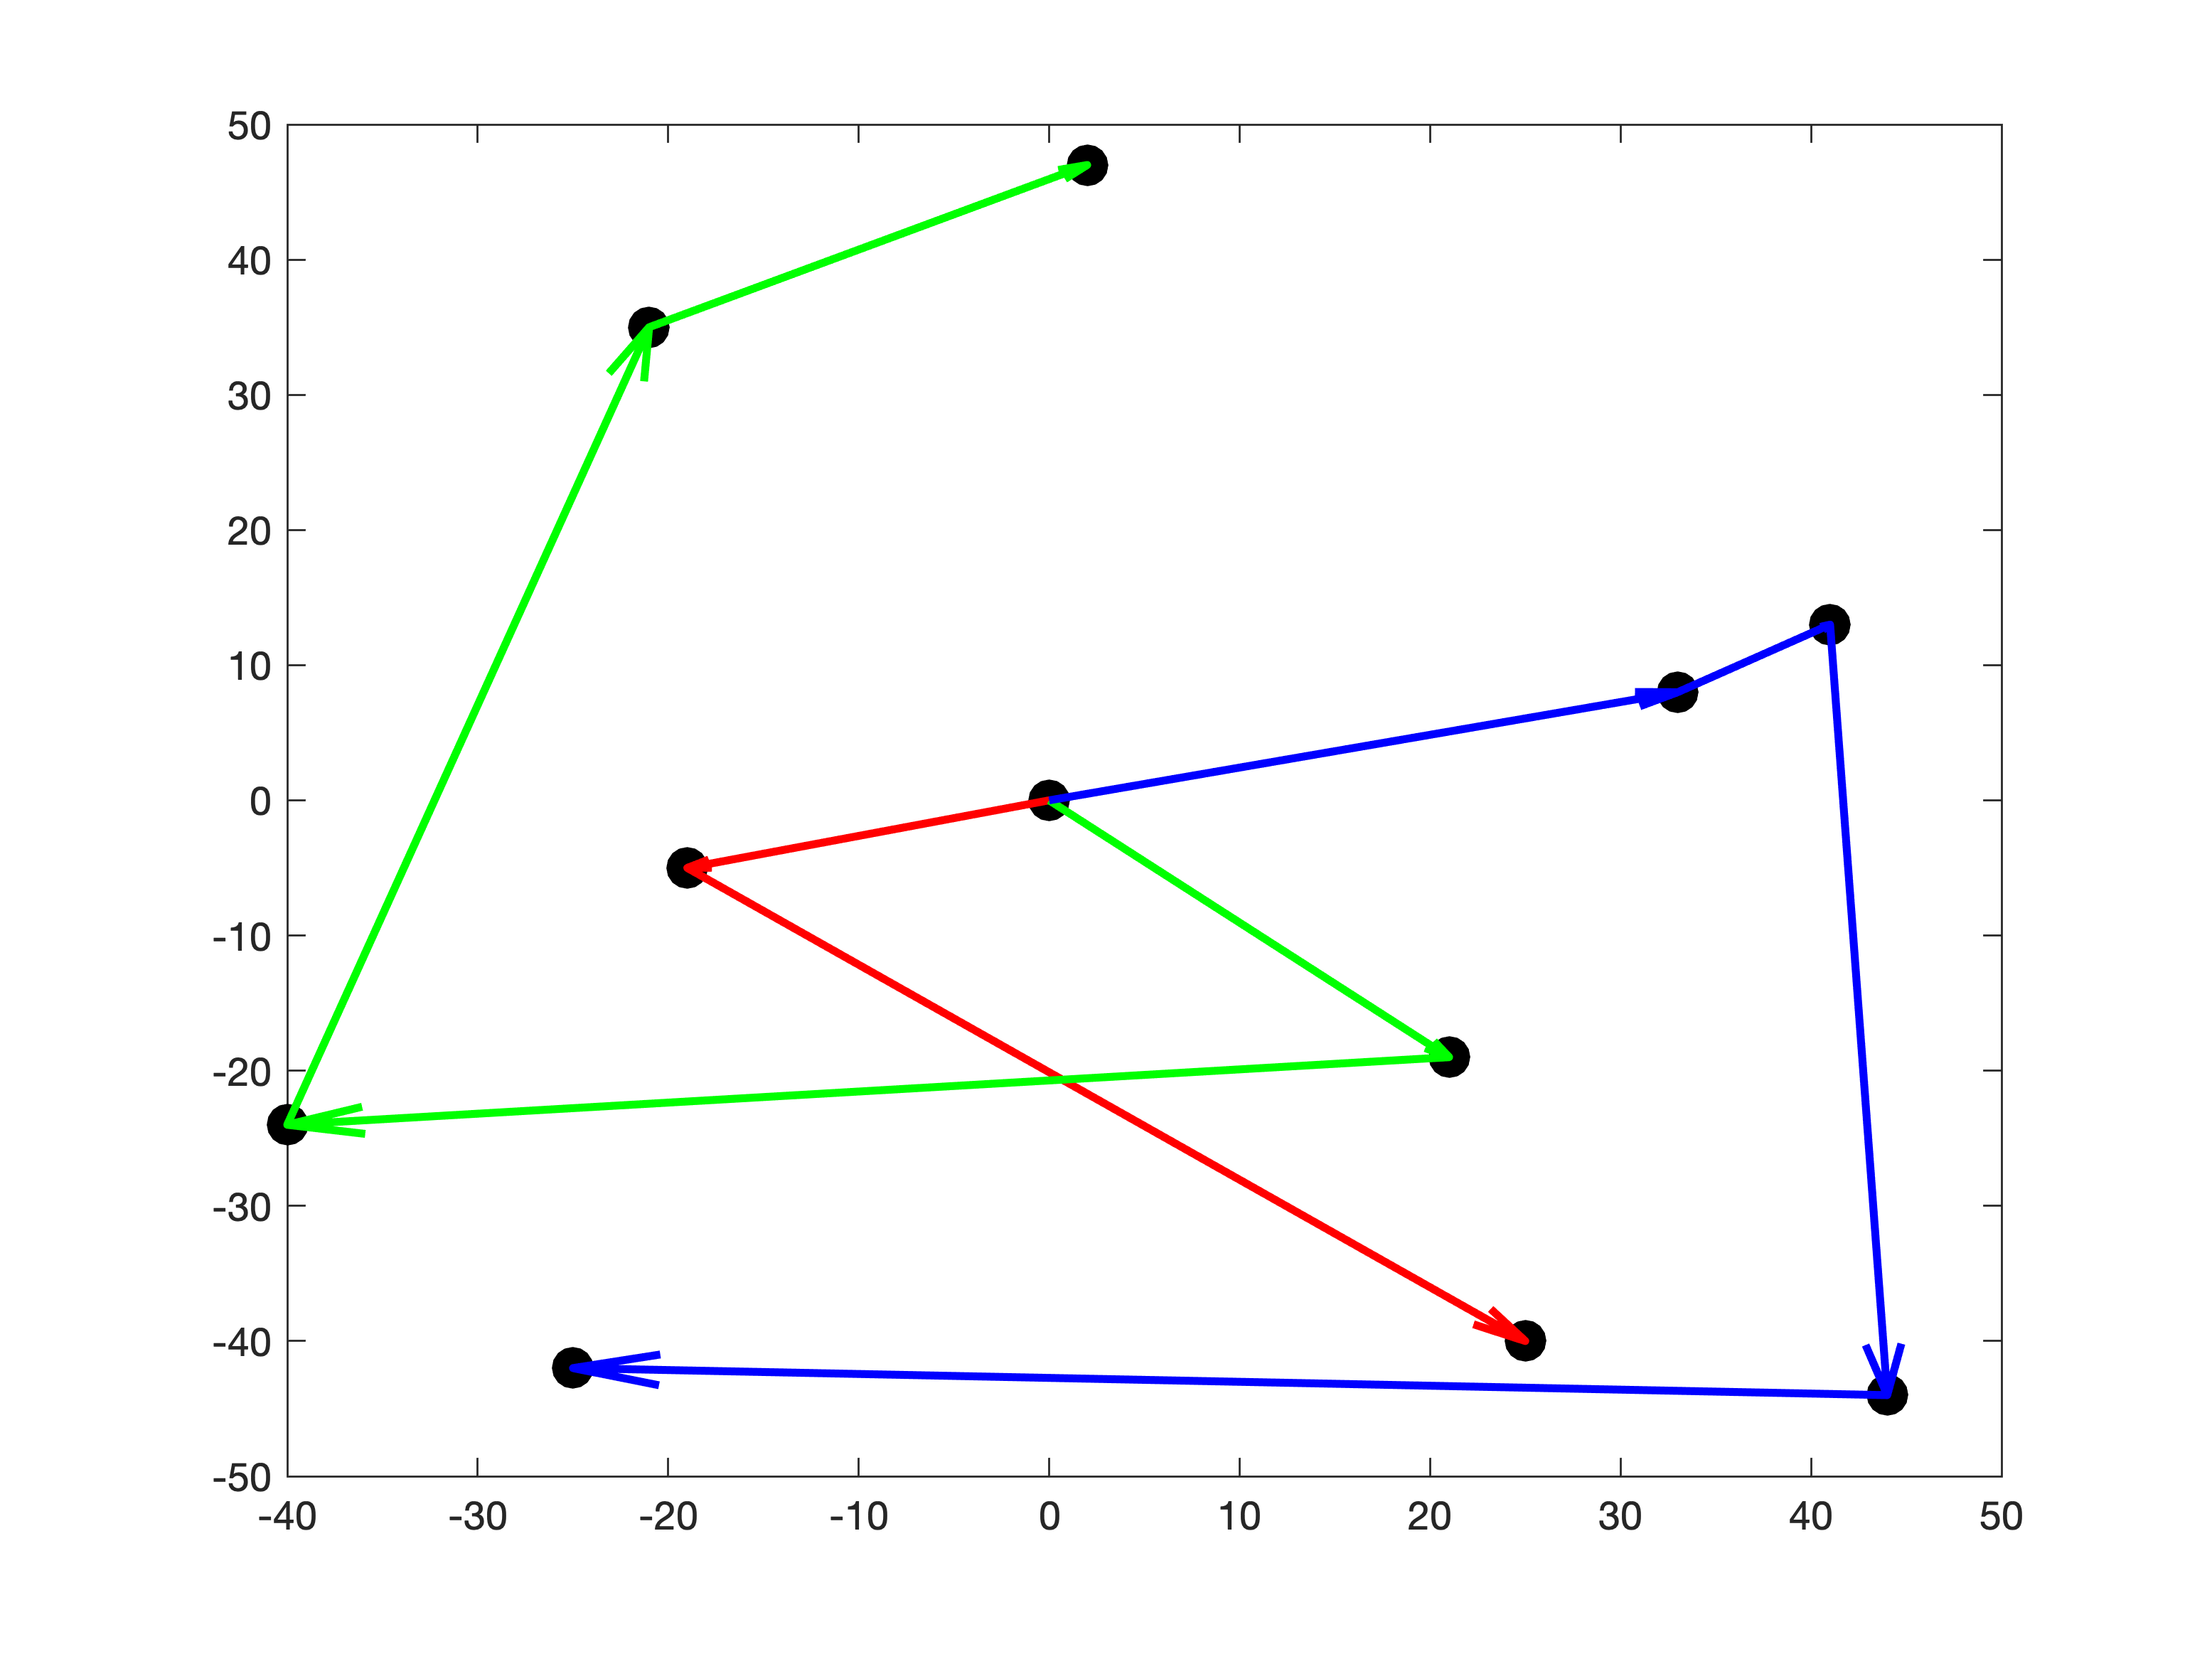
\includegraphics[width=12cm]{../Figure/Q4/best_path.png}
	\centering
	\caption{مسیر بهینه کامیونت‌ها به مراکز (هر رنگ نشان دهنده مسیر یک کامیونت است.)}
	\label{best_path_truck}
\end{figure}